\documentclass[12pt,titlepage,a4paper]{report}

% Texte
\usepackage[utf8]{inputenc}
\usepackage[T1]{fontenc}
\usepackage[french]{babel}
\usepackage{lmodern}

% Numéroter les chapitres a partir de chaque début de partie
\makeatletter\@addtoreset{chapter}{part}\makeatother

% Mise en page
\usepackage{url}
\usepackage[top=2.1cm,bottom=2cm,left=1cm,right=1cm]{geometry}
\usepackage{hyperref}
\hypersetup{
    colorlinks=false,
    pdfborder={0 0 0},
}
\usepackage{multirow}

% TOC
\usepackage[french]{minitoc}
\setcounter{tocdepth}{0}
\setcounter{minitocdepth}{2}
\setlength{\mtcindent}{0pt}

% Images
\usepackage{float}
\usepackage{wrapfig}
\usepackage{graphicx}
% Pour inclure des pages PDF
\usepackage[final]{pdfpages}	

% Algorithmique
\usepackage{algorithmeUTF8}
\usepackage{minted}

% Couverture
\usepackage{templateINSA}
\initINSA

\title{Correcteur orthographique}
\author{Antoine \bsc{Augusti}\\ Etienne \bsc{Batise}\\ Jean-Claude \bsc{Bernard}\\ Thibaud \bsc{Dauce}\\Faustine \bsc{Demiselle}}

\renewcommand\soustitre{Rapport de projet}
\renewcommand\infoBig{Projet d'Algo}
\renewcommand\infoSmall{ASI3 2013-2014}

% Les commandes utiles
\newcommand{\dictionnaire}{\textbf{Dictionnaire}}
\newcommand{\elementdico}{\textbf{ElementDictionnaire}}
\newcommand{\elementDico}{\elementdico}
\newcommand{\elementdictionnaire}{\elementdico}
\newcommand{\mot}{\textbf{Mot}}
\newcommand{\supermot}{\textbf{SuperMot}}
\newcommand{\naturelnonnul}{\textbf{NaturelNonNul}}
\newcommand{\fichierTexte}{\textbf{FichierTexte}}
\newcommand{\correcteur}{\textbf{CorrecteurOrthographique}}
\newcommand{\liste}{\textbf{Liste}}
\newcommand{\espace}[1][1]{\vspace{#1em}}
\newcommand{\listemot}{\liste$\textless$\mot$\textgreater$}
\newcommand{\listeMot}{\listemot}
\newcommand{\listesupermot}{\liste$\textless$\supermot$\textgreater$}
\newcommand{\listesuperMot}{\listesupermot}
\newcommand{\listeSuperMot}{\listesupermot}
\newcommand{\parametres}{\textbf{Parametres}}
\newcommand{\differentde}{$\ne$\ }
\newcommand{\differentDe}{$\ne$\ }
\newcommand{\infegalea}{$\leq$\ }
\newcommand{\supegalea}{$\geq$\ }

% Pour inclure du pseudo-code
\newcommand{\inputAnalyse}[1]{\input{analyse/#1.tex}}
\newcommand{\inputCP}[1]{\input{conceptionPreliminaire/#1.tex}}
\newcommand{\inputCD}[1]{\input{conceptionDetaillee/#1.tex}}

% Pour inclure du code C
\newcommand{\inputCodeH}[1]{\inputminted[tabsize=4,linenos]{c}{../programme/include/#1.h}}
\newcommand{\inputCodeC}[1]{\inputminted[tabsize=4,linenos]{c}{../programme/src/#1.c}}
\newcommand{\inputTU}[1]{\inputminted[tabsize=4,linenos]{c}{../programme/tests/test#1.c}}

\def\changemargin#1#2{\list{}{\rightmargin#2\leftmargin#1}\item[]}
\let\endchangemargin=\endlist 

\begin{document}


\titleINSA{15}{images/fond.jpg}{0}{0}{300}{\href{http://www.flickr.com/photos/lord_james/4696338852/sizes/o/in/photostream/}{\textcolor{white}{Licence CC - Lord James}}}

\dominitoc
\tableofcontents


% ######################################################################################################

\part*{Introduction}
\addcontentsline{toc}{part}{Introduction}
À la question \textit{« Pourquoi réaliser un correcteur orthographique en C ? »} nous répondons tous en coeur : « parce que on nous l'a demandé !». D'après Wikipedia, voici la définition d'un correcteur orthographique :
\begin{quote}
	« Un correcteur orthographique est, en informatique, un outil logiciel permettant d'analyser un texte afin de détecter, et éventuellement de corriger, les fautes d'orthographe et les coquilles qu'il contient. »
\end{quote}
\vspace{20px}
Le but de ce projet d'algorithmique est de réaliser un correcteur orthographique, capable de détecter des erreurs de langue à l'aide d'un dictionnaire et de proposer des corrections orthographiques pertinentes, puisées dans le dictionnaire donné.\\

Aujourd'hui tout le monde utilise au quotidien un correcteur orthographique, celui-ci étant le plus souvent déjà présent dans les smartphones et ordinateurs. Tout le monde s'est déjà fait sauver par un programme qui corrige une coquille de frappe lors de l'envoi d'un SMS ou d'un e-mail important. Un logiciel de correction orthographique ne peut pas remplacer un académicien chevronné mais permet de corriger une bonne partie des fautes d'orthographe que nous commettons, plus ou moins involontairement.\\

Pour nous aider dans la réalisation de ce projet, nous avons à notre disposition un dictionnaire de la langue française contenant plus de 300 000 mots. Ce dictionnaire doit pouvoir nous aider à proposer des corrections pertinentes pour une phrase donnée (contenant potentiellement des fautes) en argument à notre programme. Notre programme a pour objectif d'être proche du programme \textit{Aspell} du projet GNU.\\

Nous commencerons tout d'abord ce rapport par la définition des TAD utilisés ainsi que par l'analyse descendante correspondante au projet. Nous enchaînerons par la suite par la conception préliminaire puis détaillée du problème donné. Enfin nous terminerons par l'ensemble du code C de notre projet ainsi que les différents tests unitaires effectués.

% ######################################################################################################

\part{Analyse}
\chapter{TAD}
\minitoc
	\section{TAD Mot}							\inputAnalyse{TADMot}
	\section{TAD SuperMot}						\inputAnalyse{TADSuperMot}
	\section{TAD Dictionnaire}					\inputAnalyse{TADDictionnaire}

\newpage
\begin{figure}[h]
	\centering
	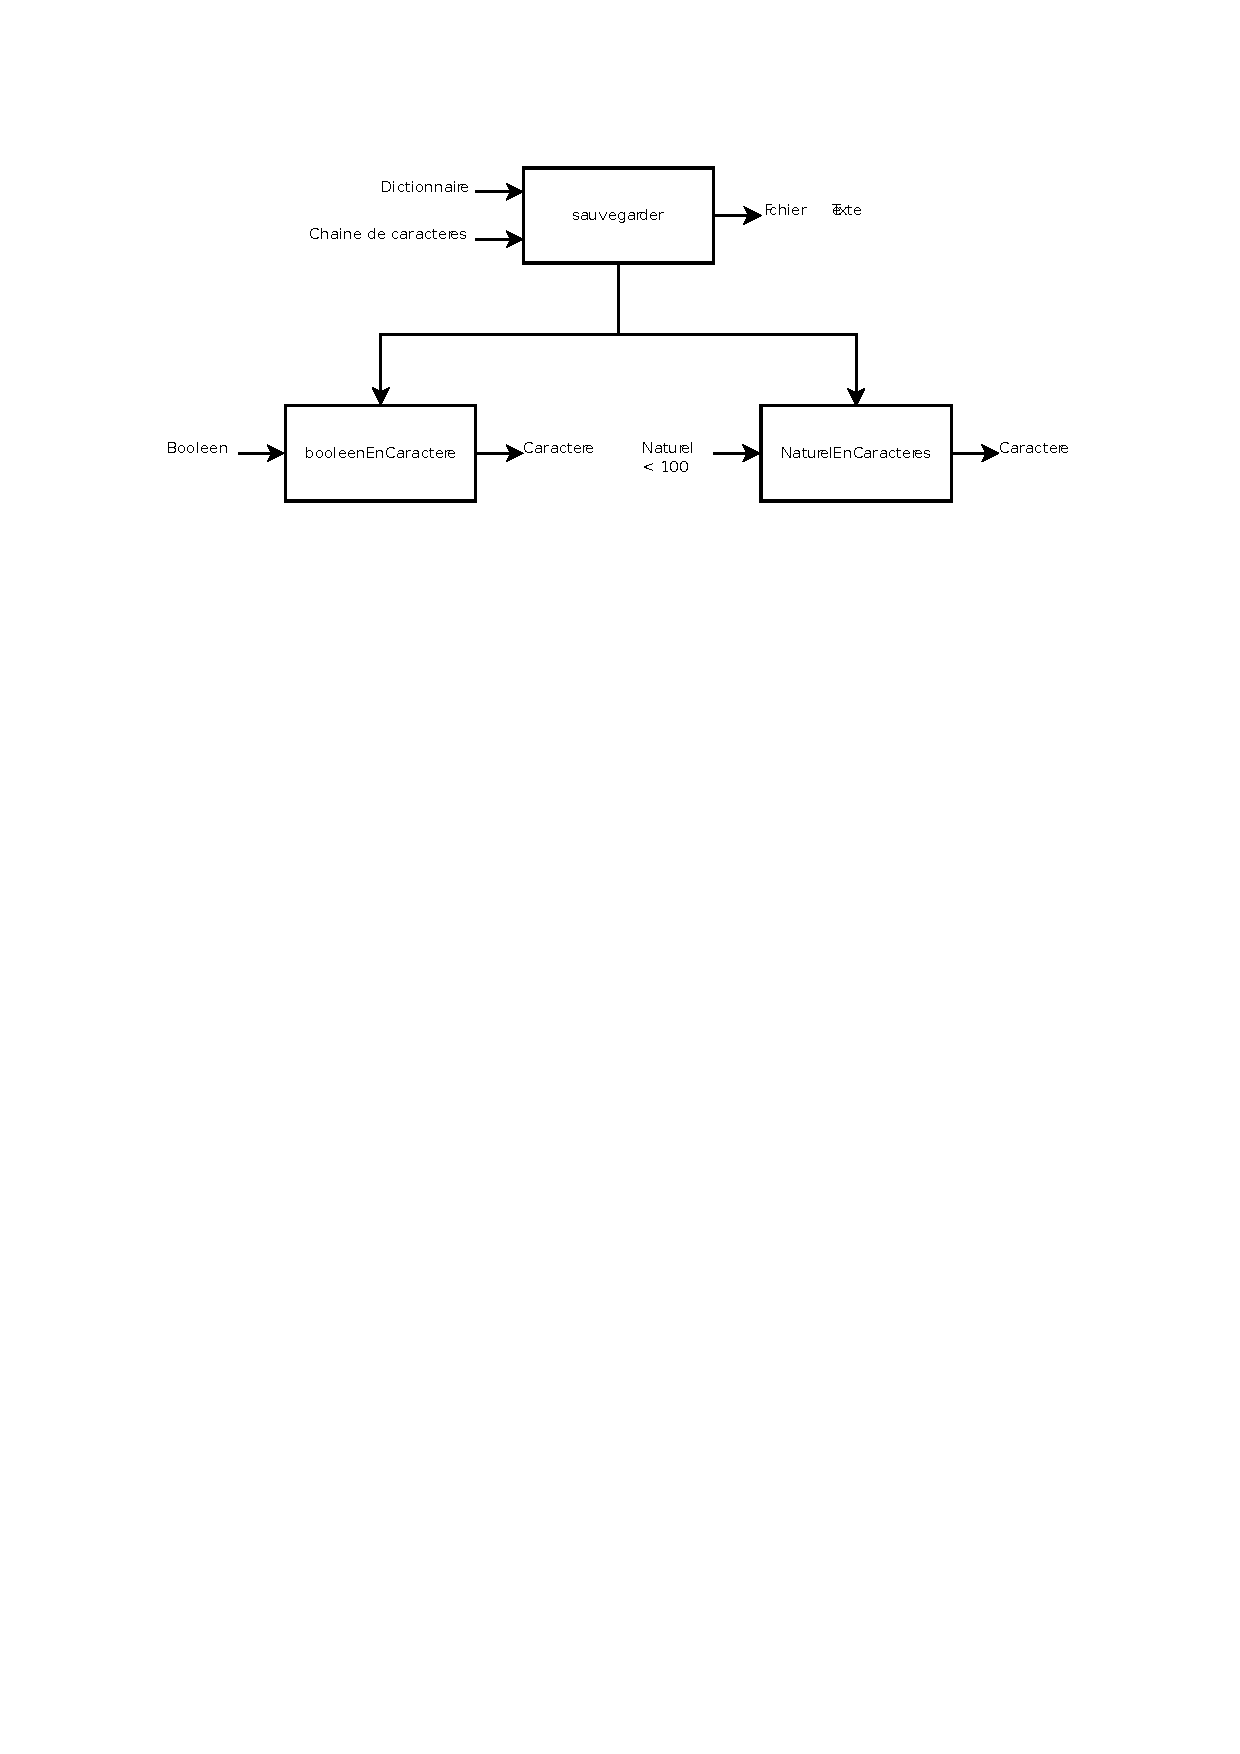
\includepdf{analyseTADDictionnaire.pdf}
	\caption{\label{analsye_descendante_TAD_dictionnaire}Analyse descendante du TAD Dictionnaire}
\end{figure}
\pagebreak

\section{TAD ElementDictionnaire}			\inputAnalyse{TADElementDictionnaire}
\section{TAD Parametres} 					\inputAnalyse{TADParametres}
\section{TAD Correcteur Orthographique}		\inputAnalyse{TADCorrecteurOrthographique}
	
\newpage
\begin{figure}
	\centering
	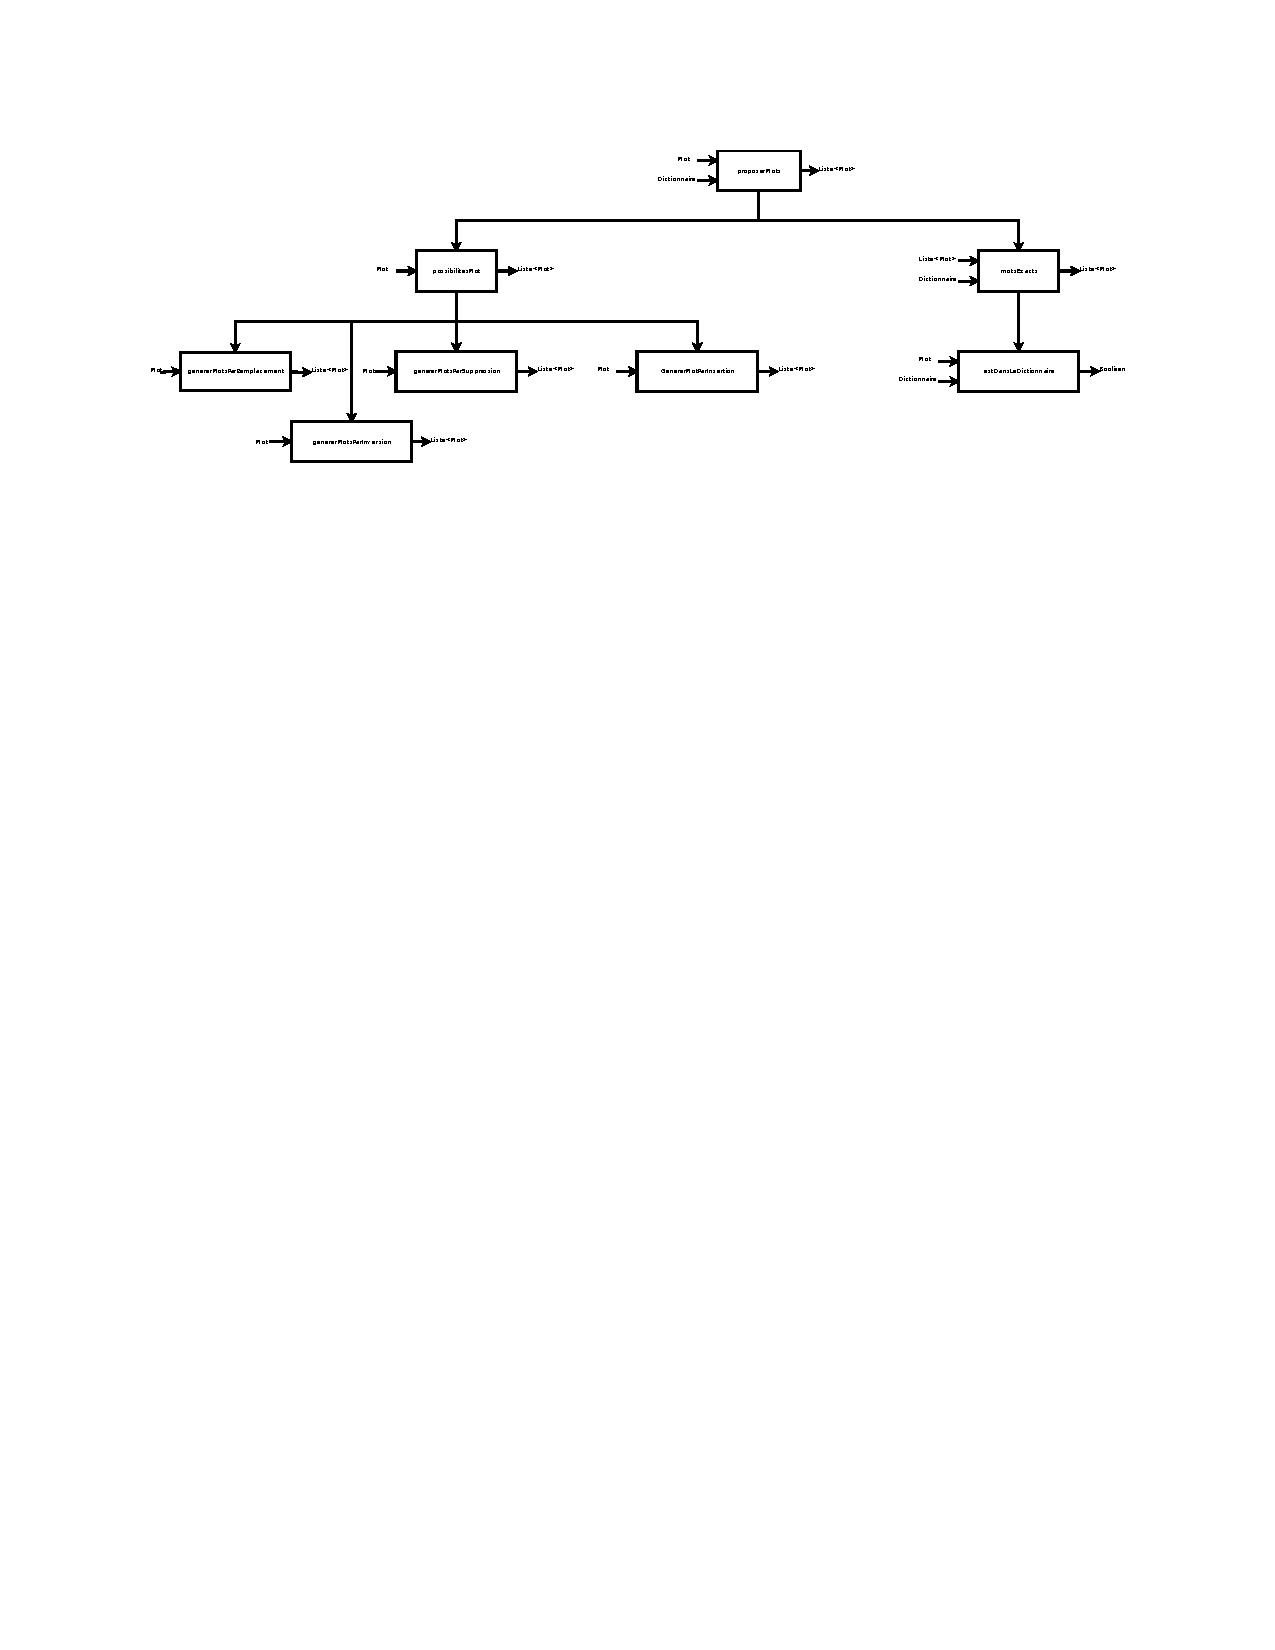
\includepdf{analyseTADCorrecteur.pdf}
	\caption{\label{analsye_descendante_TAD_correcteur}Analyse descendante du TAD Correcteur Orthographique}	
\end{figure}

\chapter{Analyse Descendante}
\begin{figure}[b]
	% 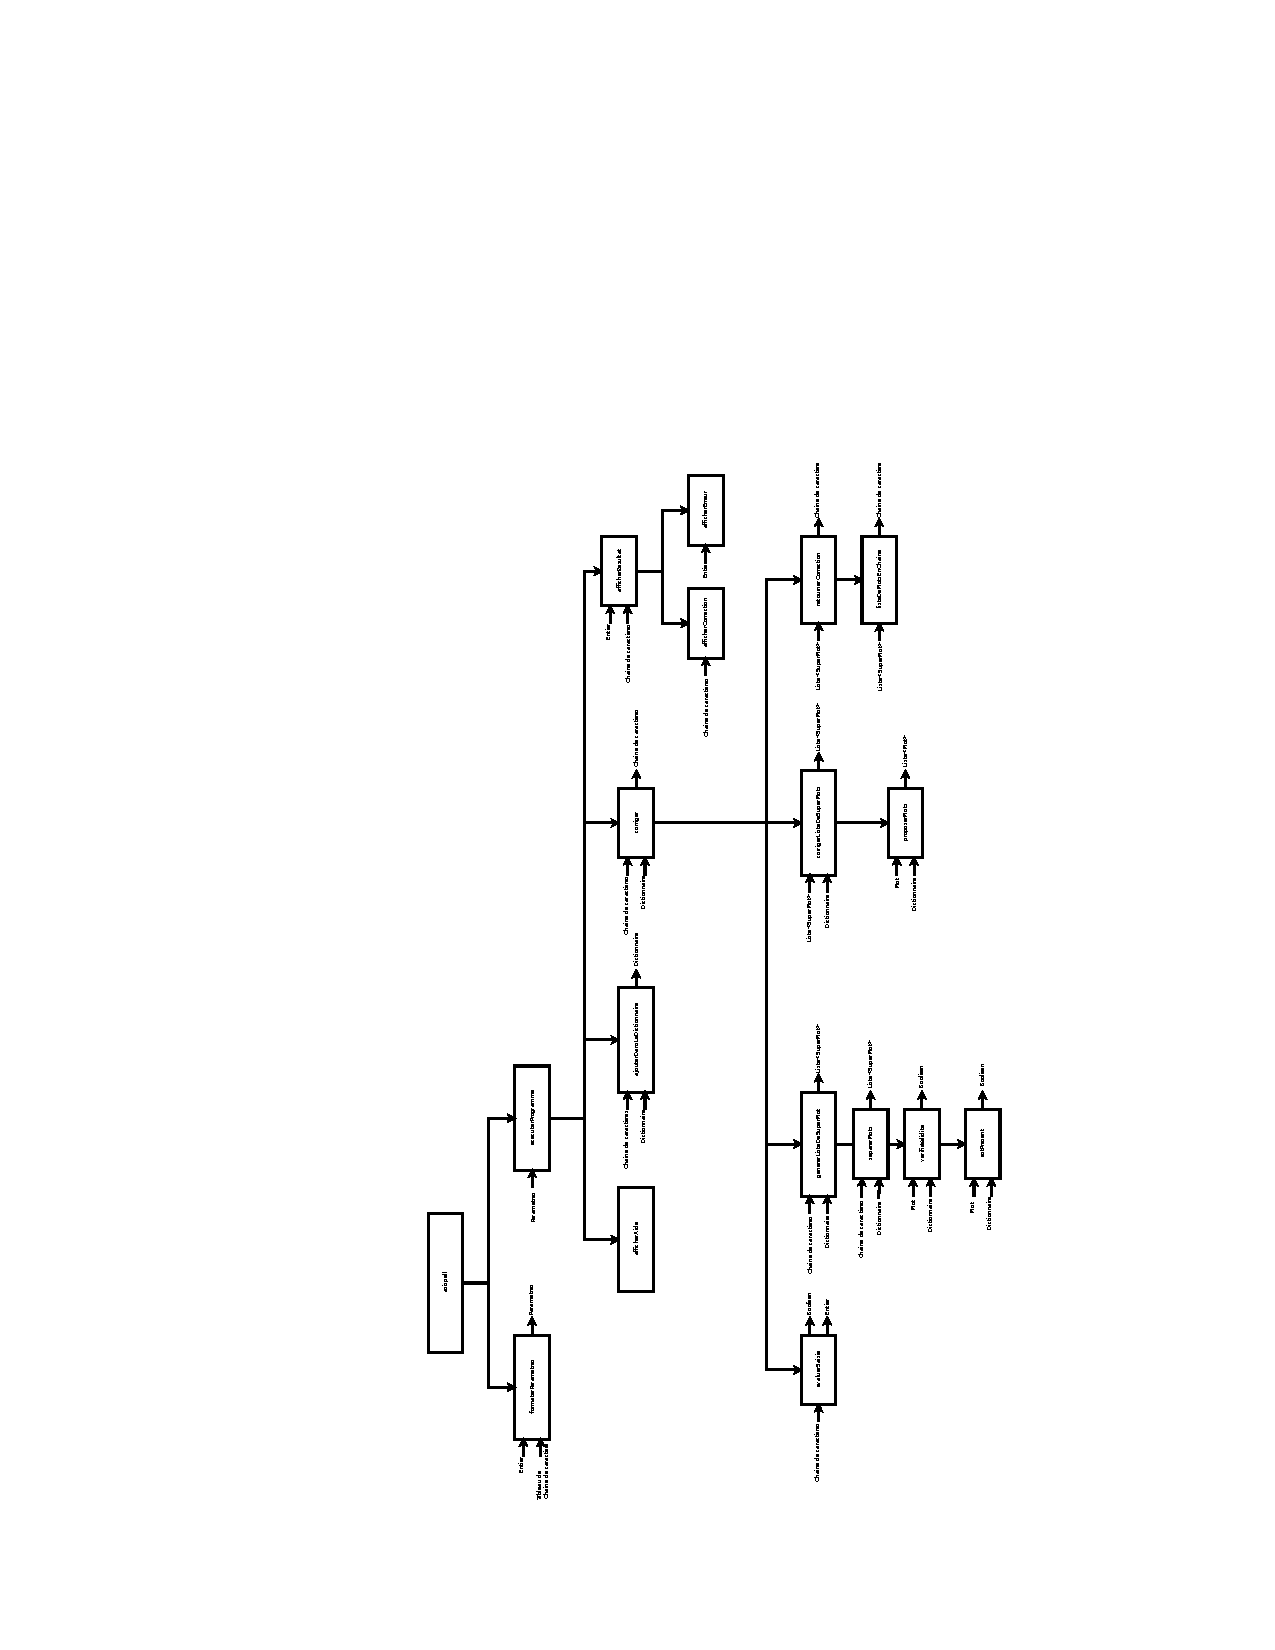
\includegraphics[scale=0.01]{analyseDescendante.pdf}	
	\centering
	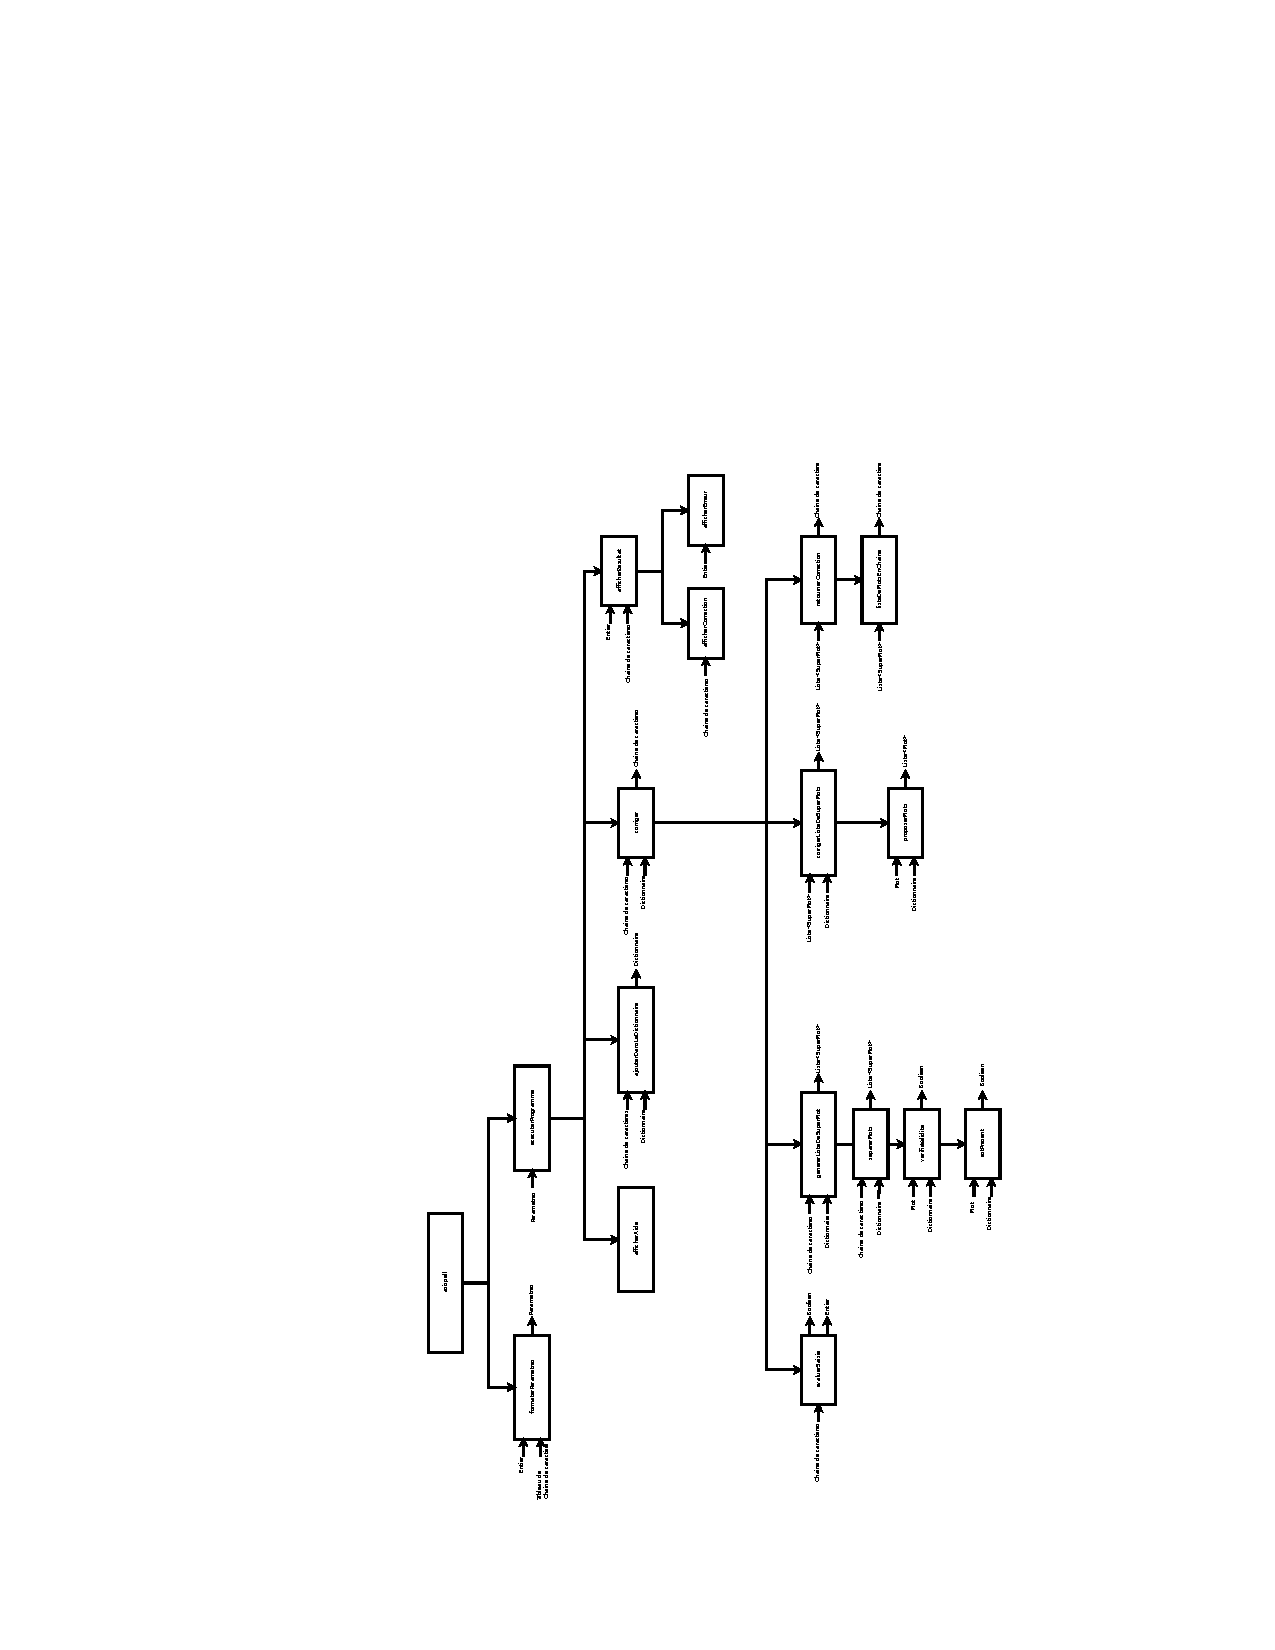
\includepdf{analyseDescendante.pdf}	
	\caption{\label{analyse_descendante}Analyse descendante du programme}
\end{figure}

% ######################################################################################################

\part{Conception préliminaire}
\chapter{Conception préliminaire des TAD}
\minitoc
	\section{TAD Mot}												\inputCP{TADMot}
	\section{TAD SuperMot}											\inputCP{TADSuperMot}
	\section{TAD Dictionnaire}										\inputCP{TADDictionnaire}
	\section{TAD ElementDictionnaire}								\inputCP{TADElementDictionnaire}
	\section{TAD Correcteur Orthographique}							\inputCP{TADCorrecteurOrthographique}
	\section{TAD Parametres}										\inputCP{TADParametres}
	
\chapter{Conception préliminaire de la logique métier}			\inputCP{logiqueMetier}	

% ######################################################################################################

\part{Conception détaillée}
\chapter{Conception détaillée des TAD}
\minitoc
	\section{TAD Mot}												\inputCD{TADMot}
	\section{TAD SuperMot}											\inputCD{TADSuperMot}
	\section{TAD Dictionnaire}										\inputCD{TADDictionnaire}
	\section{TAD ElementDictionnaire}								\inputCD{TADElementDictionnaire}
	\section{TAD Correcteur Orthographique}							\inputCD{TADCorrecteurOrthographique}
	\section{TAD Parametres}										\inputCD{TADParametres}

\chapter{Conception détaillée de la logique métier}				\inputCD{logiqueMetier}

% ######################################################################################################

\part{Code C et tests unitaires}
%% HEADERS
\chapter{Fichiers headers des TAD}
\minitoc
\section{CorrecteurOrthographique}
	\subsection{Public}					\inputCodeH{TADCorrecteurOrthographique}
	\subsection{Privé}					\inputCodeH{TADCorrecteurOrthographiquePrive}
\section{Dictionnaire}					\inputCodeH{TADDictionnaire}
\section{ElementDictionnaire}			
	\subsection{Privé}					\inputCodeH{TADElementDictionnairePrive}
\section{FichierTexte}					\inputCodeH{TADFichierTexte}
\section{ListeDeMot}					
	\subsection{Public}					\inputCodeH{TADListeDeMot}
	\subsection{Privé}					\inputCodeH{TADListeDeMotPrive}
\section{ListeDeSuperMot}					
	\subsection{Public}					\inputCodeH{TADListeDeSuperMot}
	\subsection{Privé}					\inputCodeH{TADListeDeSuperMotPrive}
\section{Mot}
	\subsection{Public}					\inputCodeH{TADMot}
	\subsection{Privé}					\inputCodeH{TADMotPrive}
\section{Parametres}					\inputCodeH{TADParametres}
\section{SuperMot}						\inputCodeH{TADSuperMot}

\chapter{Fichiers headers de la logique métier}
\minitoc
	\section{affichage}						\inputCodeH{affichage}
	\section{corriger}						\inputCodeH{corriger}
	\section{transtypage}					\inputCodeH{transtypage}

%% FICHIERS SOURCES
\chapter{Fichiers sources des TAD}
\minitoc
	\section{CorrecteurOrthographique} 		\inputCodeC{TADCorrecteurOrthographique}
	\section{Dictionnaire}					\inputCodeC{TADDictionnaire}
	\section{FichierTexte}					\inputCodeC{TADFichierTexte}
	\section{ListeDeMot}					\inputCodeC{TADListeDeMot}
	\section{ListeDeSuperMot}				\inputCodeC{TADListeDeSuperMot}
	\section{Mot}							\inputCodeC{TADMot}
	\section{Parametres}					\inputCodeC{TADParametres}
	\section{SuperMot}						\inputCodeC{TADSuperMot}

\chapter{Fichiers sources de la logique métier}
\minitoc
	\section{affichage}						\inputCodeC{affichage}
	\section{corriger}						\inputCodeC{corriger}
	\section{main}							\inputCodeC{main}
	\section{transtypage}					\inputCodeC{transtypage}

%% FICHIERS DES TUs
\chapter{Fichiers sources des tests unitaires}
\minitoc
	\section{Dictionnaire}					\inputTU{TADDictionnaire}
	\section{ElementDictionnaire}			\inputTU{TADElementDictionnaire}
	\section{FichierTexte}					\inputTU{TADFichierTexte}
	\section{ListeDeMot}					\inputTU{TADListeDeMot}
	\section{ListeDeSuperMot}				\inputTU{TADListeDeSuperMot}
	\section{Mot}							\inputTU{TADMot}
	\section{Parametres}					\inputTU{TADParametres}
	\section{SuperMot}						\inputTU{TADSuperMot}


% part code_ _c_ _et_ _tests_ _unitaires_ (end)
% ######################################################################################################
\part{Répartition du travail et conclusion}
\chapter{Conclusions personelles}
\minitoc
	\section{Antoine Augusti}
	La réalisation de ce projet algorithmique m'a permis avant tout de travailler avec un langage qui n'a pas de \textit{ramasse-miettes} au niveau de la mémoire. La gestion de la mémoire dynamique est quelque chose de complexe et j'ai trouvé la réalisation de ce projet très intéressante surtout parce que le C est un langage très sévère au niveau de la gestion de la mémoire. J'ai été également très satisfait de l'ensemble du travail de notre équipe car nous avons su tenir les délais imposés, sans chercher à avancer trop vite et sans prendre de retard.\\

	En revanche, j'étais déjà habitué à travailler sur des projets à plusieurs développeurs, avec des gestionnaires de versions et une répartition du travail entre les différentes personnes où la production d'une documentation complète est primordiale. Ce projet ne m'a donc rien appris de nouveau de ce côté car ce sont des méthodes de travail que je connais et pratique depuis plusieurs années.

	\section{Étienne Batise}
	Ce projet m'a permis tout d'abord d'apprendre à développer dans un langage rigoureux et peu permissif : le C. Il m'a permis de mieux comprendre les étapes de la compilation aussi bien que les spécificité de la gestion de la mémoire.\\

	Étant habitué à travailler sur des projets personnels en groupe, travailler avec un cahier de charges précis m'a permis d'améliorer mes capacités à m'adapter à différentes contraintes comme un calendrier prévisionnel ou des logiciels précis.

	\section{Jean-Claude Bernard}
	C'est la première fois que j'avais à réaliser un projet en C. À part en fin de lycée où j'avais commencé à apprendre le C, c'est au cours de cette année que 
	j'ai appris à compiler un programme et à gérer la mémoire. Au terme de ce projet, il s'avère que j'ai bien aimé développer en C.\\
	
	En ce qui concerne le travail de groupe, nous avons déjà été habitué à se répartir les tâches notamment avec le projet INFO et la P6. Nous nous entendions très 
	bien, nous avons avancé à notre rythme et le résultat est satisfaisant. Ce qui change des autres projets auquels j'ai participé, c'est qu'ici j'ai appris 
	à utiliser de nouveaux outils que mes camarades étaient habitués à manier.
	
	\section{Thibaud Dauce}
	Ce projet m'a permis de mettre en pratique les cours théoriques sur le C. Ce langage est bien plus complexe que ce que l'on peut croire et permet de bien comprendre comment fonctionne un ordinateur via la gestion de la mémoire, les pointeurs, etc... J'ai pu aussi utiliser pour la première fois SVN qui s'est révélé au final peu différent de Git que j'ai l'habitude d'utiliser. \\

	Cette première expérience d'une gestion de projet stricte grâce au cycle en V m'a fait peur au début, ne sachant pas si le projet allait aboutir mais s'est révélée bénéfique au final avec un programme solide à tout point de vu (analyse descendante, pseudo-code, tests unitaires...). Le travail avec mes camarades s'est bien passé, et nous avons mené le projet ensemble en suivant le calendrier prévisionnel. 

	\section{Faustine Demiselle}
	J'ai principalement appris une chose pendant ce projet : s'intégrer dans un groupe de gens qui ont l'habitude de travailler ensemble n'est pas facile. Sachant que mes camarades ont l'habitude de coder et de réaliser des projets en groupe, j'aurais peut-être dû m'investir plus et prendre plus d'initiatives. J'ai été prise de court et je me suis retrouvée à ne pas pouvoir faire ma part du travail une semaine sur l'autre car elle était déjà faite. C'est bien la première fois dans ma scolarité que ceci m'arrive.\\

	J'ai aussi appris à utiliser la banquise et son gestionnaire de versions et j'ai pu faire des progrès en C. J'ai pris la mesure de l'importance des TAD dans la réalisation d'un projet complet. 

\chapter{Conclusion générale}
\minitoc
	\section{Répartition des tâches}
	D'un point de vue de l'organisation, nous avons d'abord fait l'analyse ensemble afin de se mettre d'accord sur le rôle de chaque TAD. Puis nous avons réparti les tâches au fur et à mesure du projet, en essayant de ne pas avoir la même personne sur la même partie deux fois de suite afin de mieux détecter les erreurs. Voici comment le travail a été réparti (JC : Jean-Claude. On écrit JC parce que sinon Jean-Claude ça prend trop de place dans le tableau.) :

	\newcommand{\twoln}[1]{\multirow{2}{*}{#1}}

	\begin{center}
	\begin{tabular}
	{ |				l		||		c			|		 c		|		c		|		c			| } \hline
							&	TAD / &	Conception	&	\twoln{Dév}	&	\twoln{TU}	\\
							& CP		&	détaillée	&					&					\\ \hline \hline
		Mot							& Étienne et Faustine		& Antoine		& Thibaud	& 	JC\\ \hline
		SuperMot					& Antoine					& Antoine		& Faustine	& 	Thibaud\\ \hline
		Dictionnaire				& Thibaud et JC	& Thibaud		& Antoine et JC	& 	Étienne\\ \hline
		ElementDictionnaire			& Thibaud et JC	& JC		& Antoine et JC	& 	Faustine\\ \hline
		CorrecteurOrthographique	& Faustine					& Faustine		& Étienne	& 	-\\ \hline
		Paramètres					& Étienne 					& Étienne		& Faustine	& 	Thibaud\\ \hline
		Liste						& M. Delestre				& M. Delestre	& Étienne et Thibaud	& 	Antoine\\ \hline
		FichierTexte				& M. Delestre						& Étienne			& Étienne	& 	Étienne\\ \hline
		Logique métier				& Tous						& Tous			& Tous	& 	Tous\\ \hline
	\end{tabular}
	\end{center}

	Les fonctions de logique métier étant nombreuses et délicates en raison de la gestion de l'ensemble des TAD, nous les avons gardées pour la fin et les avons finalement partagées, c'est pourquoi tout le monde a travaillé dessus comme indiqué dans le tableau.\\

	\section{Respect du planning}
	Retrouvez dans le tableau ci-dessous le planning d'avancement prévu par M. Delestre et l'avancement réel de la réalisation de notre projet.
	\begin{center}
	\begin{tabular}
	{ |				l		||		c			|		 c		|} \hline
		Date				& Tâche prévue 				& Tâche réalisée \\ \hline \hline
		6 novembre			& TAD et rapport			& TAD et rapport	\\ \hline
		13 novembre			& Analyse descendante		& Analyse descendante	\\ \hline
		20 novembre			& CP et rapport				& CP et rapport	\\ \hline
		27 novembre			& CD et rapport				& CD et rapport	\\ \hline
		4 décembre			& Développement et TU		& CD et rapport	\\ \hline
		11 décembre			& Développement et TU		& Développement et TU	\\ \hline
		18 décembre			& Développement et TU		& Développement et TU	\\ \hline
		Vacances de Noël	& Développement et TU		& Débogage et rapport	\\ \hline
	\end{tabular}
	\end{center}

	\section{La véritable vraie conclusion}
	Pour conclure, on peut dire que ce projet est pour nous un succès tant au niveau de la réalisation que de l'organisation.\\

	D'un point de vue du travail d'équipe, nous sommes également satisfaits. Même si nous commençons à être habitués au travail d'équipe, c'était pour nous le premier véritable projet informatique d'une ampleur assez importante.\\

	Ce projet nous a permis d'apprendre comment travailler correctement en équipe sur un projet informatique, c'est-à-dire comment bien répartir le travail et comment bien s'organiser, par exemple en faisant en groupe l'analyse descendante et la conception préliminaire. Nous avons compris l'importance qu'avaient les .h et la documentation pour que tout le monde puisse savoir comment utiliser toutes les fonctions. Ainsi, nous respectons le principe d'encapsulation que l'on sait maintenant quasi primordial pour de tels projets.\\

	Nous avons également appris à utiliser de nouveaux outils adaptés à ce type de projet comme un dépôt SVN ainsi que le framework CUnit qui nous a permis de faire tous nos tests unitaires plus simplement.\\

	Enfin, ce projet aura été notre première pratique importante du C, nous ayant appris à manipuler correctement ce langage et commencer a maîtriser certaines de ses particularités et différences avec l'algorithmique.


\end{document}